\documentclass{article}

\usepackage{graphicx}

\graphicspath{./}

\begin{document}
    \title  { \textbf{SYSC 4602 Assignment 1} }
    \author {
        David Song (101071234)\\
        Ghassan Arnouk (101078550)\\
        Zachary Porter (101069001)
    }

    \maketitle

    \clearpage
    \section*{Part 3: Ethernet Frame Structure}
    \begin{figure}[htbp]
        \centering
        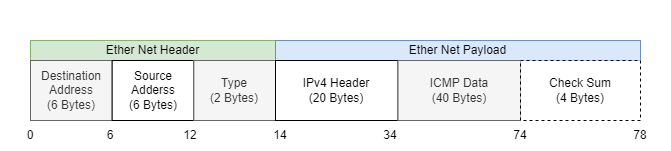
\includegraphics[width=\textwidth]{images/assignment3-part3.drawio.png}
        \caption{Ethernet Frame Structure Diagram}
        \label{fig:EthernetFrameStruct}
    \end{figure}
    As depicted in Figure \ref{fig:EthernetFrameStruct}, the Ethernet header takes up a total of 14 bytes. 6 of which are allocated for the source address, another 6 bytes for the destination address, and the remaining 2 bytes to indicate the type.

    \section*{Part 4: Protocol Overhead}
    \begin{figure}[htbp]
        \centering
        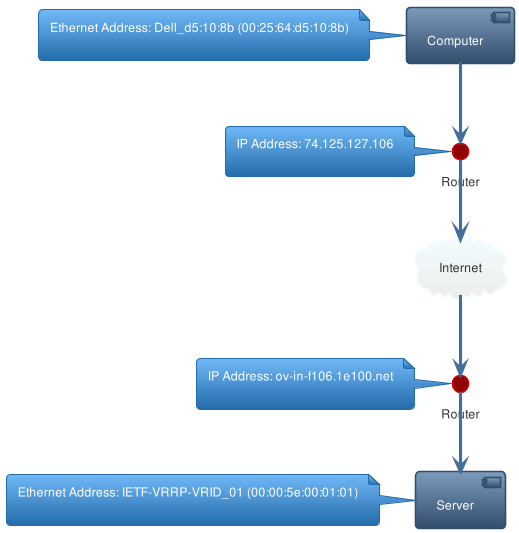
\includegraphics[width=\textwidth]{images/assignment3-part4.plantuml.png}
        \caption{Relative position of computer, router, and remote server}
    \end{figure}

    The Ethernet frame contains the physical MAC address for the source and destination addresses. The IP frame contains the IP addresses used for routing data from the source router to the destination router.

    \clearpage
    \section*{Part 5: Demultiplexing Keys}
    \subsection{What is the broadcast Ethernet address, written standard form as Wireshark displays it?}

    \subsection{Which bit of the Ethernet address is used to dethermine whether it is unicast or multicast/broadcast?}

\end{document}
